\documentclass[10pt]{beamer}

%----- 1. THEME & PACKAGES -------------------------------------------
\usetheme{journeys_econark}               % custom theme (already loads listings)
\usepackage{amsmath,amsfonts,mathrsfs}   % maths
\usepackage{textcomp}                    % symbols
\usepackage{graphicx}
\usepackage{tikz}
\usetikzlibrary{positioning,calc}
% custom listings language for YAML
\lstdefinelanguage{YAML}{
  keywords={true,false,null},
  sensitive=false,
  comment=[l]{\#},
  morestring=[b]', morestring=[b]"
}

%----- 2. METADATA ----------------------------------------------------
\title{Modular Bellman Dynamic Programming}
\subtitle{Dyn-X: Theory to High‑Dimensional Implementation}
\author[Carroll, Lujan, Shanker, White]{
  Chris Carroll (\textit{JHU}) \and Alan Lujan (\textit{JHU}) \\[0.5em]
  Akshay Shanker (\textit{UNSW/Econ-ARK}) \and Matt White (\textit{Econ-ARK})
}

\institute{\vspace{1.5em}CEF 2025}
\date{July 2025}

% custom macro
\newcommand{\Shk}{\mathfrak{S}}

%=====================================================================
\begin{document}

%---------------------------------------------------------------------
\begin{frame}
  \titlepage
\end{frame}

\begin{frame}
  \frametitle{Roadmap}
  \begin{enumerate}
    \item \textbf{Problem:} Monolithic DP code
    \item \textbf{Core Idea:} Factored Bellman → Modular CDA decomposition
    \item \textbf{Implementation:} \texttt{perches}, \texttt{movers}, and \texttt{stages}
    \item \textbf{Case Study:} Housing model with branching
    \item \textbf{Future:} Implementation, open questions \& roadmap
  \end{enumerate}
\end{frame}

%---------------------------------------------------------------------
\section{Introduction}

\begin{frame}
  \frametitle{Welcome to the 21st Century}

  \vspace{2em}
  We have clean and **modular theory** with all primitives. 

  \vspace{0.75em}
  \begin{equation*}
     \mathrm{v}_{t+1} = \mathbb T \mathrm{v}_{t}, \qquad \mathrm{v}_{t}, \mathrm{v}_{t}\in \mathcal{B}(X)
  \end{equation*}

  \vspace{2em}
  What happens when we are tasked to compute and estimate models with policy or business  applications 
  specific features? 

\end{frame}

% --- Monolithic code vs. modular decomposition -----------------------
\begin{frame}
    \frametitle{Why Is Dynamic‑Programming Code Still Monolithic?}
  
    \begin{columns}[T]
    % ---------- LEFT: pain points --------------------------------------
    \column{0.57\textwidth}
      \begin{itemize}\setlength\itemsep{4pt}
        \item \textbf{Ad hoc, one‑off, copy‑paste implementations} → near‑zero reuse.  
        \item \textbf{Curse of dimensionality $\times$ curse of idiosyncratic engineering}:  
              each new model is bespoke with handcrafted hacks.
        \item \textbf{Implications for supercomputing}: Solution structure matters.
        \item \textit{Powell (2012)}: introducing a post‑decision state  
              can "\emph{dramatically simplify}" dynamic programs —  
              yet frameworks rarely expose it.
      \end{itemize}
  

    \column{0.43\textwidth}
      \centering
      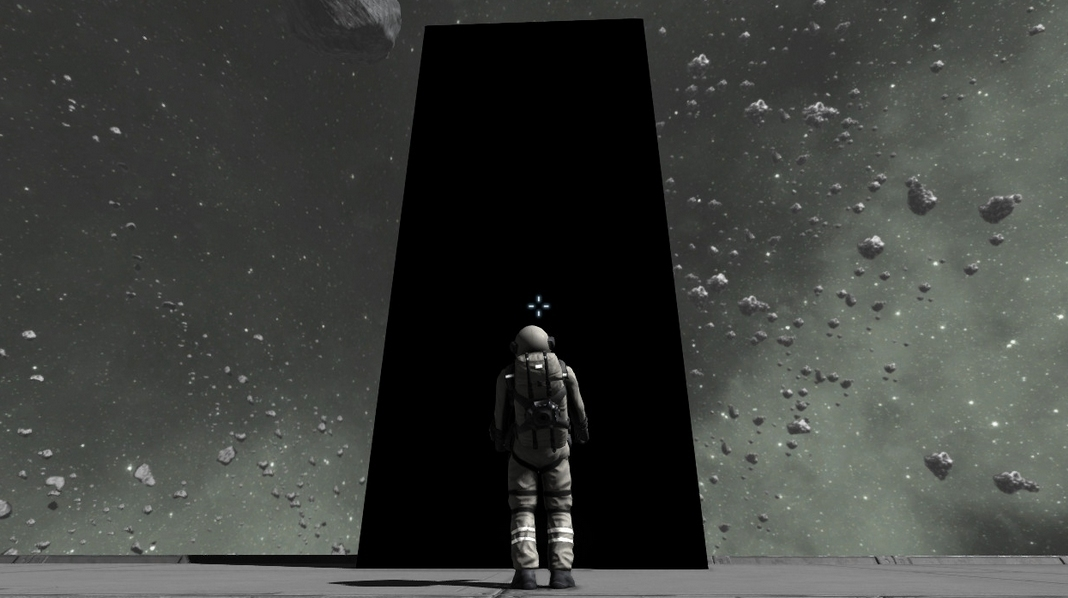
\includegraphics[width=\columnwidth, trim=350 0 350 0, clip]{space1.jpg}
  
    \end{columns}
\end{frame}

\begin{frame}[fragile]
  \frametitle{Traditional Monolithic DP}
  
  \begin{columns}[T]
    \column{0.55\textwidth}
    \begin{lstlisting}[language=Python,basicstyle=\tiny\ttfamily,numbers=none]
# All-in-one nested loops
for t in range(T-1, -1, -1):
  for i, a in enumerate(asset_grid):
    best_val = -np.inf
    for c in np.linspace(0, a, 101):
      # Utility + transition mixed
      u = np.sqrt(c)
      a_next = a - c
      j = int(round(a_next))
      # Bellman buried in loops
      val = u + beta * V[t+1, j]
      if val > best_val:
        best_val = val
    V[t, i] = best_val
    \end{lstlisting}
    
    \column{0.45\textwidth}
    \textbf{Extreme Monolith:}
    \begin{itemize}
      \item Triple nested loops
      \item State dynamics entangled with optimization
      \item Hard to modify or extend 
      \item No real operator representation
    \end{itemize}
  \end{columns}
  
  \vspace{0.5em}
  \vspace{0.6em}
  \begin{block}{Our premise}
    \centering
    \textit{Operator theoretic approach \alert{reduces mathematical complexity}, it should also reduce computational complexity.}
  \end{block}
\end{frame}

\begin{frame}[fragile]
  \frametitle{Modular Approach}
  
  \begin{columns}[T]
    \column{0.55\textwidth}
    \begin{lstlisting}[language=Python,basicstyle=\tiny\ttfamily,numbers=none]
# Separate operators for each decision
def cntn_to_dcsn(EV_next, model):
  # Backward: optimize consumption
  ...
  return V_dcsn

def dcsn_to_arvl(V_dcsn, model):
  # Backward: integrate over shocks
  ...
  return V_arvl

# Clean operator composition
T_stage = dcsn_to_arvl(cntn_to_dcsn(...))
    \end{lstlisting}
    
    \column{0.45\textwidth}
    \textbf{Main ideas:}
    \begin{itemize}
      \item Recursive problem decomposed into three operations. 
      \item Explicitly define operations as flexible computational objects and \alert{remove reference to time} within stage.
      \item Compose operators into canonical stages.
      \item Dynamic program turns out to be a \alert{graph} where operator arguments are nodes (\texttt{perches}) and operations are edges (\texttt{movers})
    \end{itemize}
  \end{columns}
  
  \vspace{-4.5em}
  \small
  Bellman factored: $\mathscr{T}^F = \mathscr{T}^{va} \circ \mathscr{T}^{ev}$
\end{frame}



\begin{frame}
  \frametitle{From Primal to Factored Bellman}
  \textbf{Primal:} Mixes action with future shock
  \[
    V_{t+1}(x)=\max_{a\in A(x)}
    \Bigl\{\,r(x,a)+\beta\,\mathbb E\bigl[V_{t}\!\bigl(f(x,a,W_{t+1})\bigr)\bigr]\Bigr\}
  \]
  \,
  \,
  where $V_{t+1}$ is the value function at time $t+1$ and $V_{t}$ is the value function at time $t$, $A(x)$ is the action set at state $x$, $r(x,a)$ is the reward function, $f(x,a,W_{t+1})$ is the transition function, and $W_{t+1}$ is the shock at time $t+1$.
 
 \vspace{1.5em}
 
\end{frame}
 
\begin{frame}
  \textbf{Factored:} Separate transitions and continuation value
  \[
    x_e=g_{ve}(x_v,a),\quad x_{v}'=g_{av}(x_e,W'), \quad \mathscr E(x_e)=\mathbb E_{W'}[\,V(x_{v}')\,]
  \]
  \[
    V(x_v)=\max_{a}\bigl\{\,r(x_v,a)+\beta\,\mathscr E\!\bigl(g_{ve}(x_v,a)\bigr)\bigr\}
  \]
  
\begin{block}{Key: Post-Decision State}
  $x_e$ = Powell's post-decision state — no nested expectation inside max
\end{block}
\end{frame}

\begin{frame}
  \frametitle{CDA State Types}
  \centering
  \begin{tabular}{lll}\hline
    \textbf{Label} & \textbf{Timing} & \textbf{Carries value} \\ \hline
    Arrival   $x_a$ & start (pre‑shock) & $\mathscr A(x_a)$ \\
    Decision  $x_v$ & post‑shock        & $\mathscr V(x_v)$ \\
    Continuation $x_e$ & post‑action   & $\mathscr E(x_e)$ \\ \hline
  \end{tabular}

  \vspace{0.8em}
  Operators: $\mathscr T^{ev}$ (optimise), $\mathscr T^{va}$ (expectation).
\end{frame}

\begin{frame}
  \frametitle{Theory Meets Implementation}
  \begin{columns}[T]
    \column{0.5\textwidth}
    \textbf{Mathematical Decomposition:}
    \[
      \boxed{\mathscr T^{F}= \mathscr T^{va}\circ \mathscr T^{ev}}
    \]
    \[
      \begin{cases}
        (\mathscr T^{ev}\mathscr E)(x_v)=\max_{a}\{r+\beta\mathscr E\}\\
        (\mathscr T^{va}\mathscr V)(x_a)=\mathbb E_W[\mathscr V(g_{av})]
      \end{cases}
    \]
    
    \column{0.5\textwidth}
    \textbf{Computational Needs:}
    \begin{itemize}
      \item Store functions \& policies
      \item Swap solvers (VFI/EGM)
      \item Connect stages
      \item Enable simulation
    \end{itemize}
  \end{columns}
  
  \vspace{0.5em}
  \begin{block}{Solution}
    Map mathematical objects directly to computational structures
  \end{block}
\end{frame}





%---------------------------------------------------------------------
\section{StageCraft Implementation}

\begin{frame}
  \frametitle{\texttt{Perches} \& \texttt{Movers}: Computational Objects}
  
  \begin{columns}[T]
    \column{0.48\textwidth}
    \textbf{\texttt{Perches} (nodes):}
    \begin{itemize}
      \item \texttt{arvl}: $\mathscr A$, $\mu_a$
      \item \texttt{dcsn}: $\mathscr V$, policy, $\mu_v$
      \item \texttt{cntn}: $\mathscr E$, $\mu_e$
    \end{itemize}
    
    \column{0.48\textwidth}
    \textbf{\texttt{Movers} (edges):}
    \begin{itemize}
      \item Backward: $\mathscr{T}^{ev}$, $\mathscr{T}^{va}$
      \item Forward: push distributions
      \item Swap solvers via config
    \end{itemize}
  \end{columns}
  
  \vspace{0.5em}
  Each \texttt{perch} stores \texttt{.sol}, \texttt{.dist}, \texttt{.grid}
\end{frame}

\begin{frame}[fragile]

A stage is a union of two direct acyclic graphs (DAGs) with \texttt{perches} as nodes and \texttt{movers} as edges. 

  \frametitle{CDA Graph Template}
\begin{lstlisting}[numbers=none,basicstyle=\ttfamily\small,frame=none]
arvl --shock--> dcsn --action--> cntn
 ^                              |
 |------- Bellman backward -----|
\end{lstlisting}
  Graph \emph{is} the composition $\mathscr T^{va}\!\circ\!\mathscr T^{ev}$. 
\end{frame}

% --- CDA Cycle (value vs. measure flows) -----------------------------
\begin{frame}[fragile]
    \frametitle{CDA Cycle — One \texttt{Stage}}
  
    \centering
    \begin{tikzpicture}[>=stealth,
        scale=0.75, transform shape,
        node distance=26mm,
        perch/.style={draw,rounded corners=1pt,
                      minimum height=9mm,minimum width=22mm,
                      font=\footnotesize,fill=OBSIDIAN_CODE_BG}]
      % -----------------------------------------------------------------
      % NODES
      \node[perch]                       (arvl) {arvl};
      \node[perch,right=of arvl]         (dcsn) {dcsn};
      \node[perch,right=of dcsn]         (cntn) {cntn};
  
      % -----------------------------------------------------------------
      % BACKWARD VALUE FLOW (dashed, pointing into/out of boxes - TOP)
      \draw[->,dashed,thick,color=OBSIDIAN_SECONDARY]
        ([yshift=3pt]cntn.west) -- node[above,font=\scriptsize]{$\mathscr T^{ev}$} ([yshift=3pt]dcsn.east);
      
      \draw[->,dashed,thick,color=OBSIDIAN_SECONDARY]
        ([yshift=3pt]dcsn.west) -- node[above,font=\scriptsize]{$\mathscr T^{va}$} ([yshift=3pt]arvl.east);
  
      % -----------------------------------------------------------------
      % FORWARD MEASURE FLOW (solid, pointing into/out of boxes - BOTTOM)
      \draw[->,thick,color=OBSIDIAN_PRIMARY]
        ([yshift=-3pt]arvl.east) -- node[below,font=\scriptsize]{$\mu_a \circ g_{av}^{-1}$} ([yshift=-3pt]dcsn.west);
  
      \draw[->,thick,color=OBSIDIAN_PRIMARY]
        ([yshift=-3pt]dcsn.east) -- node[below,font=\scriptsize]{$\mu_v \circ g_{ve}^{-1}$} ([yshift=-3pt]cntn.west);
    \end{tikzpicture}
  
    \vspace{0.8em}
    \tiny
    \textcolor{OBSIDIAN_SECONDARY}{Dashed} = Bellman (value) recursion;  
    \textcolor{OBSIDIAN_PRIMARY}{solid} = push-forward of measures.  
    This template underlies every Dyn‑X \texttt{stage}.
  \end{frame}
  



\begin{frame}
  \frametitle{\texttt{Stage} Lifecycle}
  
  %
  \begin{enumerate}\itemsep3pt
    \item Load YAML $\;\Rightarrow$ symbolic model
    \item Compile $\;\Rightarrow$ NumPy/JIT functions \& grids
    \item Solve backward via \textbf{Horse} (solver engine) + \textbf{Whisperer} (orchestrator)
    \item Simulate forward (horse)
  \end{enumerate}
  %
  \vspace{0.5em}
  \begin{block}{Clean Separation}
    \begin{itemize}
      \item \textbf{Model specification} (YAML/config) is separate from \textbf{solution algorithm}
      \item Horse = pluggable solver (VFI, EGM, etc.)
      \item Whisperer = coordinates solving across \texttt{stages}
    \end{itemize}
  \end{block}
\end{frame}

\begin{frame}
  \frametitle{GPU in Dyn‑X: Why It's Almost Free}

  \begin{itemize}\setlength\itemsep{4pt}
    \item \textbf{Thin operators}  
          each mover $\approx$ one NumPy/Numba kernel  
          $\;\Rightarrow$ launch exactly the same kernel on a GPU array
    \item \textbf{No global state}  
          per‑stage data live in \lstinline|perch.sol|  
          $\;\Rightarrow$ host $\leftrightarrow$ device copy is local, automated
    \item \textbf{Zero code change}  
          Switch backends via config: CPU $\leftrightarrow$ GPU $\leftrightarrow$ MPI\\
          Unlike ad-hoc GPU implementations
    \item \textbf{Tailored kernels}  
          Custom CUDA for Bellman max (not generic autodiff)\\
          Handles non-differentiable policies, discrete choices
  \end{itemize}

  \vspace{0.6em}
  Outcome in the housing benchmark  
  {\small(10k wealth × 30 housing × 5 income points):}
  \[
    \text{run‑time:}\; 74\text{ s (CPU)} \;\;\to\;\; 2.6\text{ s (1 V100)}
  \]
  \textbf{$\sim$30× speedup} — comparable to specialized GPU codes, but modular
\end{frame}









%---------------------------------------------------------------------
\section{Case Study: Housing Model}

\begin{frame}[fragile]
  \frametitle{YAML Excerpt}
\begin{lstlisting}[language=YAML]
state_space:
  decision: [assets, y, house]
  arrival:  [assets, house]
functions:
  utility: "alpha*np.log(c)+(1-alpha)*np.log(kappa*(house+1))"
\end{lstlisting}
  StageCraft infers the CDA graph automatically.
\end{frame}

\begin{frame}
  \frametitle{Five Housing \texttt{Stages}}
  \begin{enumerate}\itemsep2pt
    \item TENU  — tenure choice (branching)
    \item OWNH — owner housing stock
    \item RNTH — renter housing services
    \item OWNC — owner consumption (EGM)
    \item RNTC — renter consumption (EGM)
  \end{enumerate}
\end{frame}

%---------------------------------------------------------------------
\subsection{Branching \& Discrete Choice}

\begin{frame}
  \frametitle{Branching Bellman — Tenure Choice}
  Decision state $(a,H,y)$:
  \[
    V_v(a,H,y)=\max\!\Bigl\{
      V_e^{\text{rent}}\!\bigl((1+r)a+H,y\bigr),\;
      V_e^{\text{own}}(a,y,H)
    \Bigr\}.
  \]
  Arrival update:
  \[
    V_a(a,H,\bar y)=
      \mathbb E_{\xi}\bigl[V_v\bigl(a,H,f(\bar y,\xi)\bigr)\bigr].
  \]
  \begin{itemize}
    \item Rent branch liquidates housing $\Rightarrow w=(1+r)a+H$.
    \item Both continuations stored in \lstinline|cntn.sol| under keys
          \texttt{"rent"}, \texttt{"own"}.
  \end{itemize}
\end{frame}

\begin{frame}[fragile]
  \frametitle{Branching \texttt{Stage} Graph (single \texttt{cntn} perch)}

  \centering
  \begin{tikzpicture}[>=stealth, 
      scale=0.7, transform shape,
      node distance=24mm,
      perch/.style={draw,rounded corners=1pt,minimum height=7mm,
                    minimum width=20mm,font=\footnotesize,
                    fill=OBSIDIAN_CODE_BG}]
    % nodes for the branching stage
    \node[perch] (arvl) {arvl};
    \node[perch,right=of arvl] (dcsn) {dcsn};
    \node[perch,right=of dcsn] (cntn) {cntn};
    
    % nodes for next stages (own and rent)
    \node[perch,above right=15mm and 20mm of cntn] (own_arvl) {own:arvl};
    \node[perch,below right=15mm and 20mm of cntn] (rent_arvl) {rent:arvl};

    % intra-stage forward arrow (single edge)
    \draw[->,thick,color=OBSIDIAN_PRIMARY]
      (arvl) -- node[above,font=\scriptsize]{shock} (dcsn);
    \draw[->,thick,color=OBSIDIAN_PRIMARY]
      (dcsn) -- node[above,font=\scriptsize]{choice} (cntn);
    
    % inter-stage forward arrows (branching after cntn)
    \draw[->,thick,color=OBSIDIAN_PRIMARY!70!black]
      (cntn.north east) to[bend left=20] 
      node[above,font=\scriptsize]{if own} (own_arvl.west);
    \draw[->,thick,color=OBSIDIAN_PRIMARY!70!black]
      (cntn.south east) to[bend right=20] 
      node[below,font=\scriptsize]{if rent} (rent_arvl.west);
      
    % backward arrows (multiple incoming to cntn)
    \draw[->,dashed,thick,color=OBSIDIAN_SECONDARY!70!black]
      (own_arvl.west) to[bend left=20]
      node[below,font=\scriptsize]{$\mathscr{A}_{\text{own}}$} (cntn.north east);
    \draw[->,dashed,thick,color=OBSIDIAN_SECONDARY!70!black]
      (rent_arvl.west) to[bend right=20]
      node[above,font=\scriptsize]{$\mathscr{A}_{\text{rent}}$} (cntn.south east);
  \end{tikzpicture}
  \vspace{0.5em}
  
  \small
  Forward: Single path within \texttt{stage}, branches after \texttt{cntn}.\\
  Backward: Multiple value functions aggregate at \texttt{cntn}.
\end{frame}







\begin{frame}
  \frametitle{Discrete Choice — Renter Housing}
  Decision state $(w,y)$ with discrete grid $\mathbb H$:
  \[
    \mathscr T^{ev}\mathscr E(w,y)=
      \max_{\substack{S\in\mathbb H\\P^rS\le w}}
      \mathscr E\!\bigl(S,y,w-P^rS\bigr).
  \]
  Budget feasibility $P^r S\le w$ is enforced in the choice set.
\end{frame}

\begin{frame}[fragile]
  \frametitle{YAML Snippet — Discrete Choice}
\begin{lstlisting}[language=YAML]
dcsn_to_cntn:
  type: forward
  method: discrete_choice
  choice_grid:
    S: {type: linspace, min: S_min, max: S_max, points: S_pts}
constraints:
  - "P_r*S <= w"
\end{lstlisting}
  The backward \lstinline|cntn_to_dcsn| mover enumerates the $S$‑grid
  (stored in \lstinline|cntn.grid["S"]|) and takes the element‑wise $\max$.
\end{frame}



%---------------------------------------------------------------------
\subsection{Stage Links \& Results}


  




  









%---------------------------------------------------------------------
\section{Conclusion}

\begin{frame}
  \frametitle{Solver Toolkit \& Simulation}
  \begin{columns}[T]
    \column{0.55\textwidth}
    \textbf{Solver Methods:}
    \begin{itemize}
      \item \textbf{VFI} + GPU (30× speedup)
      \item \textbf{EGM} (Carroll 2006)
      \item \textbf{DCEGM} (Iskhakov et al. 2017)
      \item \textbf{FUES} (4× fewer grid points)
    \end{itemize}
    
    \column{0.45\textwidth}
    \textbf{Forward Simulation:}
    \small
    \texttt{arvl.dist} → \texttt{dcsn.dist} → \texttt{cntn.dist}
    
    \vspace{0.5em}
    Mass preserved at each step
  \end{columns}
  
  \vspace{0.5em}
  \begin{block}{Key: Swap solvers via config, not code}
  \end{block}
\end{frame}



\begin{frame}
  \frametitle{Why Not Use Existing Tools?}
  
  \begin{columns}[T]
    \column{0.48\textwidth}
    \textbf{Generic ML Frameworks:}
    \begin{itemize}
      \item TensorFlow/JAX: Arrays \& ops
      \item No economic primitives
      \item Generic autodiff $\neq$ EGM
    \end{itemize}
    
    \column{0.48\textwidth}
    \textbf{Economics Libraries:}
    \begin{itemize}
      \item HARK: Modular but not graph
      \item Dolo: DSL but no factoring
      \item QuantEcon: Solvers not stages
    \end{itemize}
  \end{columns}
  
  \vspace{0.5em}
  \begin{block}{Dyn-X: Economic objects as nodes, operators as edges}
  \end{block}
\end{frame}

\begin{frame}
  \frametitle{Open Questions \& Future Work}
  
  \textbf{Core conjectures:}
  \begin{itemize}
    \item \textbf{Universality:} Any MDP → CDA form?
    \item \textbf{Minimality:} Are irreducible stages truly minimal?
    \item \textbf{Edge cases:} Simultaneous shocks, non-period models
  \end{itemize}
  
  \textbf{Scaling up:}
  \begin{itemize}
    \item \textbf{Heterogeneous agents:} Multiple circuits in parallel
    \item \textbf{General equilibrium:} Link circuits via market clearing
    \item \textbf{Infinite horizon:} Period structure with stationary shocks
  \end{itemize}
  
  \begin{block}{Empirical validation: 30× speedup on housing model}
  \end{block}
\end{frame}

\begin{frame}
  \frametitle{Roadmap}
  \begin{itemize}
    \item \textbf{GPU via Numba CUDA} (implemented, 30× speedup)
    \item \textbf{MPI} for distributed computing
    \item \textbf{JAX/cuPy backends} (planned)
    \item \textbf{Lean-4 export} for formal verification
  \end{itemize}
  
  \vspace{0.5em}
  \begin{block}{Dyn-X 1.0 beta: Q4 2025 — github.com/econ-ark/dynx}
  \end{block}
\end{frame}

\begin{frame}
  \frametitle{Key Takeaways}
  
  \begin{itemize}
    \item \textbf{Problem:} Monolithic DP code — no reusability
    \item \textbf{Solution:} Factored Bellman → CDA stages
    \item \textbf{Implementation:} Graph of economic objects
    \item \textbf{Performance:} 30× speedup with GPU
  \end{itemize}
  
  \vspace{1em}
  \begin{block}{Impact}
    Focus on economics, not implementation\\
    Dyn-X 1.0 beta: Q4 2025
  \end{block}
\end{frame}

\begin{frame}
  \frametitle{Thank You}
  Questions \& discussion.

  \vspace{1em}
  Slides \& code → \texttt{github.com/akshay-shanker/dynx-cef-2025}
\end{frame}

%=====================================================================
\appendix

\begin{frame}
  \frametitle{Modular MDP — Formal Definition}
  \begin{block}{Tuple}
    \[
      \bigl((\Omega,\Sigma,\mathbb P),\,J,\,
             \{\mathcal X_j\},\,
             \{\mathcal F_{\mathcal X_j}\},\,
             \{\Shk_j,\tilde\Shk_j\},\,
             \{\text{CDC}_j\}\bigr)
    \]
  \end{block}
  \vspace{-0.5em}
  \begin{enumerate}\itemsep2pt
    \item $J$: stage indices (finite or countable)
    \item $\mathcal X_j$: topological vector space of states
    \item $\mathcal F_{\mathcal X_j}\subseteq \mathscr M(\mathcal X_j,\mathbb R)$
    \item Shocks $\Shk_j$ (observable) and $\tilde\Shk_j$ (latent)
    \item $\text{CDC}_j:\mathcal F_{\mathcal X_{j+1}}\!\to\!\mathcal F_{\mathcal X_j}$
  \end{enumerate}
  
  Stage $j$ is \emph{irreducible} if $\sigma(\Shk_j)$ and $\sigma(\tilde\Shk_j)$ admit no non-trivial independent sub-algebras.
\end{frame}

\begin{frame}
  \frametitle{Complex Example: Mortgage Model with Sub-Circuits}
  
  \centering
  \begin{tikzpicture}[>=stealth, 
      scale=0.65, transform shape,
      node distance=14mm and 18mm,
      perch/.style={draw,rounded corners=1pt,minimum height=8mm,
                    minimum width=18mm,font=\scriptsize,
                    fill=OBSIDIAN_CODE_BG}]
    
    % === PERIOD 0 ===
    % Tenure choice
    \node[perch,fill=OBSIDIAN_SUCCESS!20!OBSIDIAN_CODE_BG] (tc0) at (0,0) {TC};
    \node[below=1mm of tc0,font=\scriptsize] {Tenure Choice};
    
    % Renter branch (top)
    \node[perch,fill=OBSIDIAN_PRIMARY!20!OBSIDIAN_CODE_BG] (r0) at (2.5,2) {R};
    \node[below=1mm of r0,font=\scriptsize] {Renter};
    
    % Owner branch (bottom)
    \node[perch,fill=OBSIDIAN_ALERT!20!OBSIDIAN_CODE_BG] (ha0) at (2.5,-2) {HA};
    \node[below=1mm of ha0,font=\scriptsize] {Housing Adj};
    
    \node[perch] (kh0) at (5,-1) {KH};
    \node[below=1mm of kh0,font=\scriptsize] {Keep House};
    
    \node[perch] (ah0) at (5,-3) {AH};
    \node[below=1mm of ah0,font=\scriptsize] {Adjust House};
    
    % Consumption/Mortgage stage
    \node[perch,fill=OBSIDIAN_SECONDARY!20!OBSIDIAN_CODE_BG] (cm0) at (7.5,0) {CM};
    \node[below=1mm of cm0,font=\scriptsize] {Cons/Mortgage};
    
    % === PERIOD 1 ===
    % Tenure choice
    \node[perch,fill=OBSIDIAN_SUCCESS!20!OBSIDIAN_CODE_BG] (tc1) at (11,0) {TC};
    \node[below=1mm of tc1,font=\scriptsize] {Tenure Choice};
    
    % Renter branch (top)
    \node[perch,fill=OBSIDIAN_PRIMARY!20!OBSIDIAN_CODE_BG] (r1) at (13.5,2) {R};
    \node[below=1mm of r1,font=\scriptsize] {Renter};
    
    % Owner branch (bottom)
    \node[perch,fill=OBSIDIAN_ALERT!20!OBSIDIAN_CODE_BG] (ha1) at (13.5,-2) {HA};
    \node[below=1mm of ha1,font=\scriptsize] {Housing Adj};
    
    \node[perch] (kh1) at (16,-1) {KH};
    \node[below=1mm of kh1,font=\scriptsize] {Keep House};
    
    \node[perch] (ah1) at (16,-3) {AH};
    \node[below=1mm of ah1,font=\scriptsize] {Adjust House};
    
    % Consumption/Mortgage stage
    \node[perch,fill=OBSIDIAN_SECONDARY!20!OBSIDIAN_CODE_BG] (cm1) at (18.5,0) {CM};
    \node[below=1mm of cm1,font=\scriptsize] {Cons/Mortgage};
    
    % === PERIOD 0 CONNECTIONS ===
    % Forward (solid)
    \draw[->,thick,color=OBSIDIAN_PRIMARY]
      (tc0) -- node[above,sloped,font=\scriptsize]{rent} (r0);
    \draw[->,thick,color=OBSIDIAN_PRIMARY]
      (tc0) -- node[below,sloped,font=\scriptsize]{own} (ha0);
    
    \draw[->,thick,color=OBSIDIAN_PRIMARY]
      (ha0) -- node[above,sloped,font=\scriptsize]{keep} (kh0);
    \draw[->,thick,color=OBSIDIAN_PRIMARY]
      (ha0) -- node[below,sloped,font=\scriptsize]{adjust} (ah0);
    
    \draw[->,thick,color=OBSIDIAN_PRIMARY]
      (r0) to[out=0,in=135] (cm0);
    \draw[->,thick,color=OBSIDIAN_PRIMARY]
      (kh0) to[out=0,in=180] (cm0);
    \draw[->,thick,color=OBSIDIAN_PRIMARY]
      (ah0) to[out=0,in=225] (cm0);
    
    % Backward (dashed)
    \draw[->,dashed,thick,color=OBSIDIAN_SECONDARY]
      (cm0) to[out=145,in=0] (r0);
    \draw[->,dashed,thick,color=OBSIDIAN_SECONDARY]
      (cm0) to[out=180,in=0] (kh0);
    \draw[->,dashed,thick,color=OBSIDIAN_SECONDARY]
      (cm0) to[out=215,in=0] (ah0);
    
    \draw[->,dashed,thick,color=OBSIDIAN_SECONDARY]
      (kh0) -- (ha0);
    \draw[->,dashed,thick,color=OBSIDIAN_SECONDARY]
      (ah0) -- (ha0);
    
    \draw[->,dashed,thick,color=OBSIDIAN_SECONDARY]
      (r0) -- (tc0);
    \draw[->,dashed,thick,color=OBSIDIAN_SECONDARY]
      (ha0) -- (tc0);
    
    % === PERIOD 1 CONNECTIONS ===
    % Forward (solid)
    \draw[->,thick,color=OBSIDIAN_PRIMARY]
      (tc1) -- node[above,sloped,font=\scriptsize]{rent} (r1);
    \draw[->,thick,color=OBSIDIAN_PRIMARY]
      (tc1) -- node[below,sloped,font=\scriptsize]{own} (ha1);
    
    \draw[->,thick,color=OBSIDIAN_PRIMARY]
      (ha1) -- node[above,sloped,font=\scriptsize]{keep} (kh1);
    \draw[->,thick,color=OBSIDIAN_PRIMARY]
      (ha1) -- node[below,sloped,font=\scriptsize]{adjust} (ah1);
    
    \draw[->,thick,color=OBSIDIAN_PRIMARY]
      (r1) to[out=0,in=135] (cm1);
    \draw[->,thick,color=OBSIDIAN_PRIMARY]
      (kh1) to[out=0,in=180] (cm1);
    \draw[->,thick,color=OBSIDIAN_PRIMARY]
      (ah1) to[out=0,in=225] (cm1);
    
    % Backward (dashed)
    \draw[->,dashed,thick,color=OBSIDIAN_SECONDARY]
      (cm1) to[out=145,in=0] (r1);
    \draw[->,dashed,thick,color=OBSIDIAN_SECONDARY]
      (cm1) to[out=180,in=0] (kh1);
    \draw[->,dashed,thick,color=OBSIDIAN_SECONDARY]
      (cm1) to[out=215,in=0] (ah1);
    
    \draw[->,dashed,thick,color=OBSIDIAN_SECONDARY]
      (kh1) -- (ha1);
    \draw[->,dashed,thick,color=OBSIDIAN_SECONDARY]
      (ah1) -- (ha1);
    
    \draw[->,dashed,thick,color=OBSIDIAN_SECONDARY]
      (r1) -- (tc1);
    \draw[->,dashed,thick,color=OBSIDIAN_SECONDARY]
      (ha1) -- (tc1);
    
    % === INTER-PERIOD CONNECTION ===
    \draw[->,thick,color=OBSIDIAN_PRIMARY,line width=2pt]
      (cm0) -- node[above,font=\scriptsize]{age} (tc1);
    
    % === SUB-CIRCUIT BOXES ===
    % Period 0
    \draw[thick,color=OBSIDIAN_PRIMARY,rounded corners=3pt,dashed] 
      ($(r0.south west)+(-0.3,-0.8)$) rectangle ($(r0.north east)+(0.3,0.3)$);
    
    \draw[thick,color=OBSIDIAN_ALERT,rounded corners=3pt,dashed] 
      ($(ha0.south west)+(-0.3,-0.8)$) rectangle ($(ah0.north east)+(0.3,0.3)$);
    
    % Period 1
    \draw[thick,color=OBSIDIAN_PRIMARY,rounded corners=3pt,dashed] 
      ($(r1.south west)+(-0.3,-0.8)$) rectangle ($(r1.north east)+(0.3,0.3)$);
    
    \draw[thick,color=OBSIDIAN_ALERT,rounded corners=3pt,dashed] 
      ($(ha1.south west)+(-0.3,-0.8)$) rectangle ($(ah1.north east)+(0.3,0.3)$);
    
    % Labels
    \node[above=8mm of r0,font=\footnotesize,color=OBSIDIAN_PRIMARY] {Renter Path};
    \node[below=12mm of ah0,font=\footnotesize,color=OBSIDIAN_ALERT] {Owner Path};
    
    % Period labels
    \node[above=20mm of tc0,font=\small] {\textbf{Period 0}};
    \node[above=20mm of tc1,font=\small] {\textbf{Period 1}};
  \end{tikzpicture}
  
  \vspace{0.5em}
  \tiny
  TC = Tenure Choice, R = Renter, HA = Housing Adjustment, KH = Keep House, AH = Adjust House, CM = Consumption/Mortgage\\
  Two periods showing within-period sub-circuits: renter path (blue) and owner path (red) can be solved in parallel.
\end{frame}



\end{document}
